
%!TEX encoding = UTF-8 Unicode
\documentclass{simpleslides}

\author{Björn Regnell \\ \vspace{1em}{\small \url{https://cs.lth.se/bjorn-regnell}}}
\title{An Overview of Selected\\Requirements Engineering Methods}

\date{\footnotesize Version: \today}
\begin{document}
\maketitle

\begin{frame}[fragile]{Requirements Elicitation Methods}
\begin{itemize}
\item Stakeholder analysis
\item Interviews
\begin{itemize}
  \item Unstructured interviews: open questions, open topics
  \item Structured interviews: closed questions, focused topics
  \item Semi-structured: combine both
\end{itemize}
\item Surveys
\item Group activities
\begin{itemize}
  \item Brainstorming
  \item Focus groups
  \item Demonstrations
\end{itemize}
\item Usability testing
\item Usage statistics
\item Feedback from marketing and support
\item User and developer communities
\item Mining social media
\end{itemize}
\end{frame}
  

\begin{frame}[fragile]{Requirements Specification Methods}
Different kinds of representations:
\begin{itemize}
\item Text, photos, drawings, diagrams, movies, prototypes, ...
\end{itemize}
Examples of requirements models:
\begin{itemize}
\item Static models: What exists in the domain and product?
\begin{itemize}
\item Goal models: stakeholders, goals+relations (helps, hurts)
\item System scope: context diagram, actors, interfaces
\item Data models: E/R-diagrams, Data dictionaries
\item Feature models (in text or pictures):\\why, what: functions+data, examples of how,\\expected quality,\\links to other features and models
\end{itemize}
\item Dynamic Models: What happens at runtime?
\begin{itemize}
\item Scenario-based models:\\narratives, user stories, task models, use case models
\item State-transition models: state diagrams, transition matrices
\item Test Cases: acceptance tests, system tests, unit tests
\item User interface models: mockups, GUI Designs
\item Communication protocols
\end{itemize}
\end{itemize}
\end{frame}

\begin{frame}[fragile]{Requirements Validation Methods}
\begin{itemize}
\item Inspections
\item Checklists
\item Automated checks
\item Usability testing
\item Focus groups
\item Prototyping
\item Simulation
\end{itemize}
\end{frame}
  

\begin{frame}[fragile]{Requirements Selection Methods}
What is in and what is out (for now)?
\begin{itemize}
\item Prioritization: assessing value and cost, making trade-offs
\item Road-mapping: long-term product strategy 
\item Release planning: delivery commitments under constraints
\item Being adaptable to changes in plans and strategies
\item Technical debt assessment
\end{itemize}
\end{frame}


\begin{frame}[fragile]{Requirements Validation Methods}
\begin{itemize}
\item Inspections
\item Checklists
\item Automated checks
\item Usability testing
\item Focus groups
\item Prototyping
\item Simulation
\end{itemize}
\end{frame}

\begin{frame}[fragile]{Requirements Prioritization}

\begin{itemize}
\item Examples of different aspects to rank on some scale
\begin{itemize}
  \item value: financial benefit, urgency, strategic value, market share, brand fitness, release theme, ...
  \item cost: staff effort, lead time, training, runtime costs, ... 
  \item risk: technical risk, market risk, competence risk, ...
  \item volatility: rate of change, uncertainties, ...
\end{itemize}
\item Different types of scales with different power
\begin{itemize}
  \item categorization \{A, B\}: must, ambiguous, volatile
  \item ordinal scale $A > B$: higher value, more expensive 
  \item ratio scale $A = k \cdot B$: amount of money, hours, percentage
\end{itemize}
\item Different methods, can be combined
\begin{itemize}
  \item grouping, e.g. post-it notes on a white-board
  \item select top N, e.g. N=5
  \item grading of singular requirements, e.g. 1..5, high--medium--low 
  \item ordering by pair-wise comparison (sorting)
  \item \$100-test: distribute fictitious money to reflect priority
\end{itemize}
\end{itemize}
\end{frame}

\begin{frame}[fragile]{The QUPER model: prioritizing quality requirements}
\begin{center}
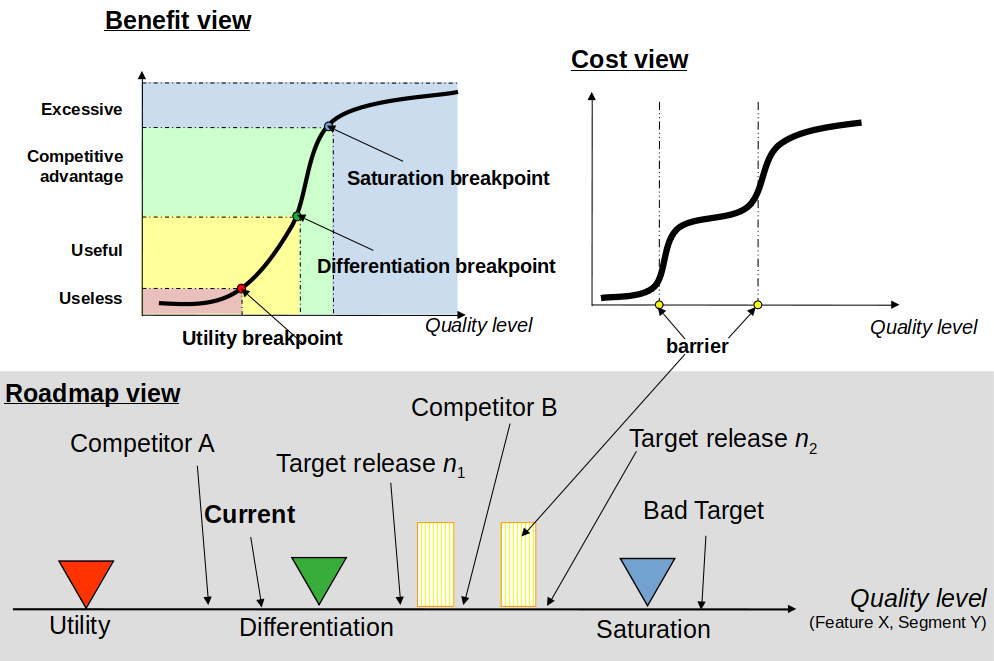
\includegraphics[width=1.0\textwidth]{img/quper}
\end{center}
{\footnotesize ''Supporting Roadmapping of Quality Requirements'' 
\\ B. Regnell, R. Berntsson Svensson, T. Olsson, \emph{IEEE} Software (2008)}
\end{frame}
  

\begin{frame}[fragile]{Written report in Requirements Enigeering}
\begin{itemize}
\item Select a topic of interest
\item Literature search
\item Read selected papers
\item Discuss with peers
\item Write report
\item Get feedback
\end{itemize}
\end{frame}

\begin{frame}[fragile]{Further studies in RE}
  Starting-points for literature search:

\begin{itemize}\footnotesize
\item \url{https://scholar.google.se/}\\
\item \url{https://cs.lth.se/bjorn-regnell/publications/}\\
\end{itemize}

\vfill
Part of preparation:
\begin{itemize}\footnotesize
  \item ''Requirements engineering challenges in market-driven
  software development -- An interview study with practitioners'' \\ L. Karlsson, Å. G. Dahlstedt, B. Regnell, J. Natt och Dag, A. Persson, \emph{Information and Software Technology} (2008) 
\end{itemize}

  Further recommended reading: 
\begin{itemize}\footnotesize
  \item ''Market-Driven Requirements Engineering for Software Products'' \\ B. Regnell, S. Brinkkemper \\ \emph{Chapter 13 in the book ''Engineering and Managing Software Requirements'' Eds. Wholin \& Aurum},  ISBN 3 540 25043 3 (2005)
  \item ''Supporting Roadmapping of Quality Requirements'' \\ B. Regnell, R. Berntsson Svensson, T. Olsson, \emph{IEEE} Software (2008) 
  \item ''Software requirements -- styles and techniques'' \\ S. Lauesen, ISBN 0 201 74570 4  (2002) 
\end{itemize}

\end{frame}


\end{document}

